\documentclass[11pt]{article}
\usepackage{amsmath, amssymb, amsthm}
\usepackage{graphicx}
\usepackage{hyperref}

\newcommand{\R}{\mathbb{R}}
\newcommand{\norm}[1]{\left\lVert #1 \right\rVert}
\DeclareMathOperator{\tr}{tr}
\newtheorem{theorem}{Theorem}

\title{Notes on Gradient Descent}
\author{Ada Lovelace \and Alan Turing}
\date{\today}

\begin{document}
\maketitle

\begin{abstract}
We review the convergence of \emph{gradient descent} on smooth convex functions and give a
short proof of the classical $O(1/k)$ rate.
\end{abstract}

\section{Introduction}\label{sec:intro}
Let $f \colon \R^n \to \R$ be convex and $L$-smooth, so that
\begin{equation}
  \norm{\nabla f(x) - \nabla f(y)} \le L \norm{x - y} \quad \text{for all } x, y. \label{eq:smooth}
\end{equation}
Gradient descent\footnote{Also called \textit{steepest descent}.} iterates
$x_{k+1} = x_k - \eta \nabla f(x_k)$ with step size $\eta = 1/L$; see \cite{nesterov}.

\subsection{Assumptions}
\begin{itemize}
  \item $f$ is \textbf{convex} and differentiable;
  \item condition~\eqref{eq:smooth} holds --- the gradient is Lipschitz;
  \item a minimizer $x^\star$ exists.
\end{itemize}

\section{Main result}\label{sec:main}
\begin{theorem}[Convergence]
After $k$ steps,
\begin{align}
  f(x_k) - f(x^\star) &\le \frac{L \norm{x_0 - x^\star}^2}{2k} \label{eq:rate} \\
  \tr(\nabla^2 f) &\le nL. \nonumber
\end{align}
\end{theorem}

Combining Section~\ref{sec:intro} with \eqref{eq:rate} gives the rate in Table~\ref{tab:rates}.

\begin{table}[htbp]
  \centering
  \caption{Rates for first-order methods}\label{tab:rates}
  \begin{tabular}{lcr}
    \hline
    Method & Rate & Memory \\
    \hline
    Gradient descent & $O(1/k)$ & $O(n)$ \\
    Accelerated & $O(1/k^2)$ & $O(n)$ \\
    \hline
  \end{tabular}
\end{table}

\begin{figure}[h]
  \centering
  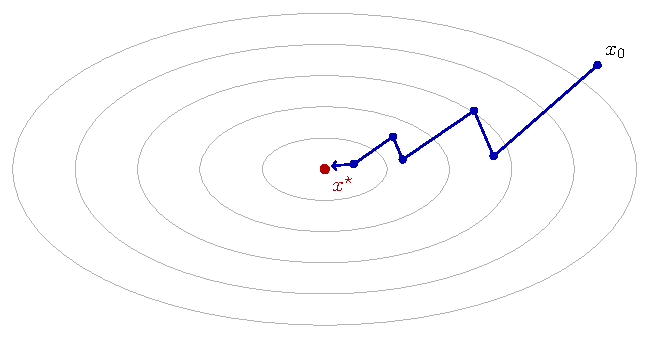
\includegraphics[width=0.6\linewidth]{figures/descent.pdf}
  \caption{Iterates of gradient descent on a quadratic.}\label{fig:path}
\end{figure}

\begin{enumerate}
  \item Pick $x_0$.
  \item Repeat until $\norm{\nabla f(x_k)} < \varepsilon$:
  \begin{enumerate}
    \item step along $-\nabla f(x_k)$;
    \item increase $k$.
  \end{enumerate}
\end{enumerate}

% A comment the reader never sees.
More at \href{https://en.wikipedia.org/wiki/Gradient_descent}{Wikipedia}. Typeset with \LaTeX.

\begin{thebibliography}{9}
\bibitem{nesterov} Y.~Nesterov. \emph{Lectures on Convex Optimization}. Springer, 2018.
\end{thebibliography}

\end{document}
